The latest version of GPGPU-Sim is a (mostly) object-oriented design written in
C++ with a sharp delineation between the functional and timing models of the
system.
A high-level overview of the organization is shown in Figure
\ref{fig:gpgpusim_top}. The SIMT blocks can be thought of as NVIDIA-like Streaming
Multiprocessors (SMs) or AMD-like Compute Units (CUs). The interconnect is currently
a modified
version of BookSim~\cite{booksim}, which can model a variety of topologies, and
the memory partition is a custom model. The remainder of this section describes
the integration of GPGPU-Sim with SST.

   \begin{figure}[!htb]
      \centering
      \setlength{\abovecaptionskip}{6pt plus 1pt minus 1pt}
      \includegraphics[width=.85\textwidth,keepaspectratio]{figures/gpgpusim_top.png}
      \captionsetup{format=hang, justification=centering, width=.75\textwidth}
      \caption[Overall GPGPU-Sim Architecture]{Overall GPGPU-Sim Architecture \protect\cite{gpgpu_sim}}
      \label{fig:gpgpusim_top}
   \end{figure}

\section{Scheduler}
\label{sec:sched}
The first step in integrating GPGPU-Sim into SST is to handle the interaction
with a SST CPU component. Since GPUs today function solely as co-processors,
functionally executing GPU-enabled binaries requires the CPU to initialize and
launch kernels of work to the GPU. In our model, the GPU is constructed out of
two discrete SST components -- a scheduler and a SM block~\cite{v100}. A block
diagram of the model is shown in Figure~\ref{fig:gpu_sched}. When CUDA functions
are called from the CPU component, they are intercepted and translated into
messages that are transfered by SST links to the GPU (along with the associated
parameters).

The CPU component (Ariel in the initial implementation) is connected via SST
links to 2 GPU components: the SMs, which implement the timing and functional
model for the GPU cores, and a centralized kernel and CTA scheduler (GPUSched).
When CUDA calls are intercepted from the CPU, messages are sent to both the SMs
and the GPU scheduler. Messages related to memory copies and other information
necessary to populate the GPU functional model are sent directly to the SM
elements, since the functional model for executing the GPU kernels lives inside
the SM elements. Calls related to enqueuing kernels for execution are sent to
the GPU scheduler element, which co-ordinates the launching of CTAs on the SMs,
{\em e.g.} \texttt{cudaConfigureCall} and \texttt{cudaLaunch}.


   \begin{figure}[!htb]
      \centering
      \setlength{\abovecaptionskip}{6pt plus 1pt minus 1pt}
      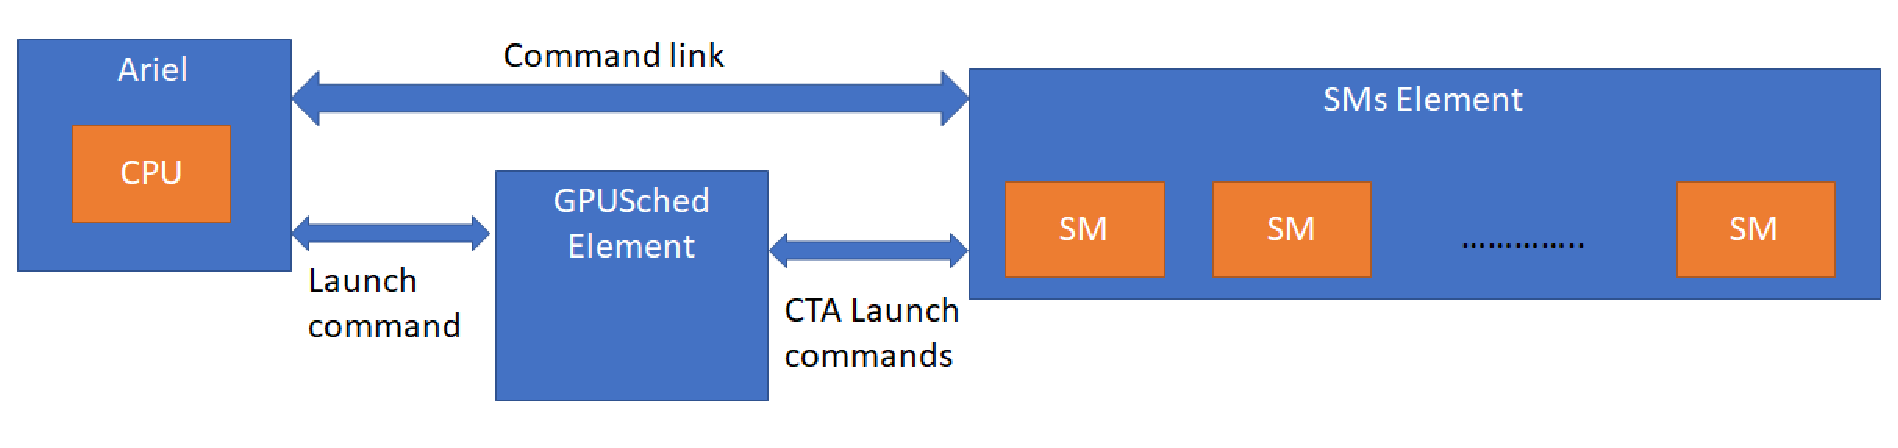
\includegraphics[width=.95\textwidth,keepaspectratio]{figures/sched.eps}
      \captionsetup{format=hang, justification=centering, width=1.0\textwidth}
      \caption{SST Element Architecture for Kernel/CTA Scheduler and SMs Components}
      \label{fig:gpu_sched}
   \end{figure}


As CTAs complete on the SMs, messages are sent back to the GPU scheduler
element, which pushes new work to the SMs from enqueued kernels as needed.
Memory copies from the CPU to GPU address space are handled on a configurable
page-size granularity, similar to how conventional CUDA unified memory handles
the transfer of data from CPU to GPU memories.


   \begin{figure}[!htb]
      \centering
      \setlength{\abovecaptionskip}{6pt plus 1pt minus 1pt}
      \includegraphics[width=.75\textwidth,keepaspectratio]{figures/scheduler.eps}
      \captionsetup{format=hang, justification=centering, width=.75\textwidth}
      \caption{Centralized GPU Scheduler Component}
      \label{fig:sched}
   \end{figure}


The centralized GPU scheduler receives kernel launch commands from the CPU, then
issues CTA launch commands to the SMs. The scheduler also receives notifications
from the SMs when the CTAs finish. The reception of kernel launch and CTA
complete notifications are independent, therefore we designed a different
handler for each type of message. Figure~\ref{fig:sched} shows the design of the
centralized kernel and CTA Scheduler. The kernel handler listens to calls from a
CPU component and pushes kernel launch information to the kernel queue when it
receives kernel configure and launch commands. The SM map table contains CTA
slots for each of the SMs, which is reserved when launching a CTA and released when a
message indicating that a CTA has finished is received from the SMs. The
scheduler clock ticks trigger CTA launches to SMs, when space is available and
there is a pending kernel. On every tick, the scheduler issues a CTA launch
command for currently unfinished kernels if any CTA slot is available or tries
to fetch a new kernel launch from kernel queue. The CTA handler also waits for
SMs to reply the CTA finish message, so that CTA slots in the SM map table may
be freed.


\section{Streaming-Multiprocessor}
\label{sec:sms}
To support the GPGPU-Sim functional model, a number of the simulator's overloaded
CUDA Runtime API calls were updated. A number of functions that originally assumed
the application and simulator were within same address space now support them being
decoupled. Initialization functions, such as \texttt{\textunderscore \textunderscore
cudaRegisterFatBinary}, now take paths to the original application to obtain the PTX
assembly of CUDA kernels.

   \begin{figure}[!htb]
      \centering
      \setlength{\abovecaptionskip}{6pt plus 1pt minus 1pt}
      \includegraphics[width=.90\textwidth,keepaspectratio]{figures/transfer_flow.png}
      \captionsetup{format=hang, justification=centering, width=.75\textwidth}
      \caption{SST Link and IPCTunnels for Functional Model Support}
      \label{fig:gpu_transfer_model}
   \end{figure}


Supporting the functional model of GPGPU-Sim also requires transferring values
from the executing CPU application to the GPU memory system. This is solved by leveraging
the inter-process communication tunnel framework from SST-Core, as shown in
Figure~\ref{fig:gpu_transfer_model}. Chunks of memory are transferred from the CPU
application to the GPU memory system at the granularity of a standard memory page (4KiB). The
transfer of pages is a blocking operation, therefore all stores to the GPU
memory system must be completed before another page is transferred or another
API call is processed.

To complete the integration with SST, everything except the SIMT units are
replaced with SST components, as shown in Figure~\ref{fig:gpgpu_sst}. The host
CPU is swapped for a SST execution component, such as Ariel or Juno. The
interconnect is swapped for a SST networking component, such as Shogun,
Kingsley, or Merlin. The memory partition, caches, and ports are swapped for
SST memHierarchy components -- caches and backing store models such as
TimingDRAM, SimpleMem, or CramSim. A detailed description of how to use the GPU
component can be found in~\cite{sst_gpgpu}. The remainder of this paper is
dedicated to a discussion of performance.


   \begin{figure}[!htb]
      \centering
      \setlength{\abovecaptionskip}{6pt plus 1pt minus 1pt}
      \includegraphics[width=.85\textwidth,keepaspectratio]{figures/sst_gpgpusim_top.png}
      \captionsetup{format=hang, justification=centering, width=.75\textwidth}
      \caption{SST GPGPU-Sim Integration}
      \label{fig:gpgpu_sst}
   \end{figure}

